\documentclass[11pt,letterpaper]{report}
\usepackage{amssymb,amsfonts,color,graphicx,amsmath,enumerate}
\usepackage{tikz}
\usepackage{amsthm}
\usepackage{bbm}

\newcommand{\naturals}{\mathbb{N}}
\newcommand{\integers}{\mathbb{Z}}
\newcommand{\complex}{\mathbb{C}}
\newcommand{\reals}{\mathbb{R}}
\newcommand{\exreals}{\overline{\mathbb{R}}}
\newcommand{\mcal}[1]{\mathcal{#1}}
\newcommand{\mable}{measurable}
\newcommand{\quats}{\mathbb{H}}
\newcommand{\rationals}{\mathbb{Q}}
\newcommand{\norm}{\trianglelefteq}
\newcommand{\Aut}{\text{Aut}}
\newcommand{\disk}{\mathbb{D}}
\newcommand{\halfplane}{\mathbb{H}}
\newcommand{\Lp}[2]{\left\|{#1}\right\|_{L^{#2}}}
\newcommand{\supp}[1]{\text{supp}({#1})}
\newcommand{\Hom}[2]{\text{Hom}_{{#1}}({#2})}
\newcommand{\tr}{\text{tr}}
\newcommand{\field}{\mathbb{F}}
\newcommand{\Gal}[1]{\text{Gal}\left({#1}\right)}
\newcommand{\esssup}{\text{ess sup }}
\newcommand{\essinf}{\text{ess inf }}
\newcommand{\affine}{\mathbb{A}}
\newcommand{\E}{\mathbb{E}}
\newcommand{\Prob}{\mathbb{P}}
\newcommand{\Var}{\text{Var}}
\newcommand{\ind}{\mathbbm{1}}
\newcommand{\Cov}{\text{Cov}}

\newenvironment{solution}
{\begin{proof}[Solution]}
{\end{proof}}

\voffset=-3cm
\hoffset=-2.25cm
\textheight=24cm
\textwidth=17.25cm
\addtolength{\jot}{8pt}
\linespread{1.3}

\begin{document}
\noindent{\em Liam Hardiman\hfill{November 27, 2019} }
\begin{center}
{\bf \Large 271A - Homework 5}
\vspace{0.2cm}
\hrule
\end{center}

\noindent\textbf{Problem 1. }
Consider the space $\reals^d$ and the usual $\|\cdot \|_2$ metric. Show explicitly that a probability measure $\Prob$ on the measurable space $(\reals^d, \mcal{B}(\reals^d))$ is uniquely determined by
\[
F(x_1, \ldots, x_d) = \Prob[y: y_1\leq x_1, \ldots, y_d\leq x_d].
\]
\begin{proof}
	Our strategy is to use the $\pi$-$\lambda$ theorem. Suppose $\Prob_1$ and $\Prob_2$ are two probability measures that agree on sets of the form $\{y_1 \leq x_1, \ldots, y_d\leq x_d)$. Define the collection $\Pi$ by
	\[
	\Pi = \big\{ \{y: y_1\leq x_1, \ldots, y_d\leq x_d\}: x\in \reals^d\big\}.
	\]
	That is, $\Pi$ consists of all products of rays. As our notation suggests, $\Pi$ is a $\pi$-system since it is clearly nonempty and the intersection of any two products of rays is again a product of rays. We also define the collection $\Lambda$ to be the sets in $\sigma(\Pi)$, the $\sigma$-algebra generated by $\Pi$, on which $\Prob_1$ and $\Prob_2$ agree:
	\[
	\Lambda = \{E \in \sigma(\Pi): \Prob_1(E) = \Prob_2(E)\}.
	\]
	This collection is indeed well-defined since every set in $\Pi$ is a Borel set, so $\sigma(\Pi)\subseteq \mcal{B}(\reals^d)$ and each $E\in \sigma(\Pi)$ is $\Prob_1$ and $\Prob_2$ measurable. We again claim that our notation makes sense and that $\Lambda$ is a $\lambda$-system. Let's verify this claim.
	\begin{itemize}
		\item $\reals^d\in \Lambda$: We can write $\reals^d$ as a union of ray-products, $\reals^d = \bigcup_{n=1}^\infty (-\infty, n]^d$, so $\reals^d$ is indeed in $\sigma(\Pi)$. That $\Prob_1[\reals^d] = \Prob_2[\reals^d]$ follows from the fact that $\Prob_1$ and $\Prob_2$ are probability measures.

		\item Closure under complements: Let $E\in \Lambda$. Since $\Prob_1$ and $\Prob_2$ are probability measures, we can write
		\[
		\Prob_1[E^c] = 1 - \Prob_1[E] = 1-\Prob_2[E] = \Prob_2[E^c].
		\]

		\item Closure under countable disjoint union: Let $\{E_n\}_{n=1}^\infty$ be a countable disjoint family in $\Lambda$. By countable additivity of measure, we have
		\[
		\Prob_1(\cup_{n=1}^\infty E_n) = \sum_{n=1}^\infty \Prob_1[E_n] = \sum_{n=1}^\infty \Prob_2[E_n] = \Prob_2(\cup_{n=1}^\infty E_n).
		\]
	\end{itemize}
	Hence, $\Lambda$ is a $\lambda$-system. By the $\pi$-$\lambda$ theorem, $\sigma(\Pi)\subseteq \Lambda$. By construction, we also have $\Lambda\subseteq \sigma(\Pi)$, so $\Lambda = \sigma(\Pi)$. But the products of rays generate all of $\mcal{B}(\reals^d)$, so we must have $\Prob_1 = \Prob_2$ on all of $\mcal{B}(\reals^d)$.
\end{proof}

\noindent\textbf{Problem 2. }
Show that if a set $A$ of continuous paths on $[0,1]$ is equicontinuous at each point in $[0,1]$ then the set is uniformly equicontinuous.
\begin{proof}
	Suppose the family is not uniformly equicontinuous but still equicontinuous at each point in $[0,1]$. Then there is some $\epsilon>0$ such that for all $n\in \naturals$, there is some $f_n\in A$ and $x_n, y_n\in [0,1]$ so that $|x_n-y_n|<1/n$ but
	\begin{equation}\label{contra}
	|f_n(x_n)-f_n(y_n)|\geq 2\epsilon.
	\end{equation}
	Since $[0,1]$ is compact, there is a subsequence $n_k$ so that $x_{n_k}\to x^*$. Since $|x_{n_k} - y_{n_k}|<1/n_k$, we have that $y_{n_k}\to x^*$ as well.\\

	\noindent Now by equicontinuity, there is some $\delta>0$ so that $|x^*-x|<\delta$ implies that $|f(x^*)-f(x)|<\epsilon$ for all $f\in A$. Choose $K$ large enough so that both $|x_{n_k} - x^*|$ and $|y_{n_k} - x^*|$ are both less than $\delta$ for all $k>K$. For $k>K$ we then have
	\begin{align*}
		|f(x_{n_k}) - f(y_{n_k})| &\leq |f(x_{n_k}) - f(x^*)| + |f(x^*) - f(y_{n_k})|\\
		&< \epsilon + \epsilon\\
		&= 2\epsilon.
	\end{align*}
	But this contradicts (\ref{contra}), so we conclude that $A$ must be uniformly equicontinuous.
\end{proof}

\noindent\textbf{Problem 3. }
Let $\zeta_i$, $i = 1, 2, \ldots$ be iid with finite first, second, and fourth moments, and consider the random walk $S_n = \sum_{i=1}^n\zeta_i$. Define the process $Y_t$ by interpolating $S_n$ as follows:
\[
Y_t = \sum_{i=1}^{\lfloor t\rfloor}\zeta_i + (t - \lfloor t\rfloor)\zeta_{i+1}.
\]
By properly rescaling and normalizing, construct a family of processes that converges in distribution to a standard Brownian motion.
\begin{solution}
	Suppose $\Var[\zeta_i] = \sigma^2$. Define the sequence of processes $X^{(m)}_t$ by
	\[
	X^{(m)}_t = \frac{1}{\sigma\sqrt{m}}Y_{mt}.
	\]
	We showed in class that $X^{(m)}$ converges in distribution to a standard Brownian motion and we'll recap some of the details here.\\

	\noindent We need to show that the family of processes $X^{(m)}$ is tight and that its finite dimensional distributions converge weakly to those of Brownian motion. 
\end{solution}

\noindent\textbf{Problem 4. }
Suppose $\{X_n\}_{n=1}^\infty$ is a sequence of random variables taking values in a metric space $(S_1, \rho_1)$ and converging in distribution to $X$. Suppose $(S_2, \rho_2)$ is another metric space, and $\phi: S_1\to S_2$ is continuous. Show that $Y_n = \phi(X_n)$ converges in distribution to $Y = \phi(X)$.
\begin{proof}
	Since $X_n \to X$ in distribution, we have that for all bounded continuous $f: S_1\to \reals$,
	\begin{equation}\label{dist}
	\E[f(X_n)] \to \E[f(X)].
	\end{equation}
	Now let $g$ be any bounded continuous function $g: S_2\to \reals$. Since $\phi$ is continuous, so is $g\circ \phi$, and since $g$ is bounded, so is $g\circ \phi$. The composition $g\circ \phi$ is then a bounded continuous function $S_1\to \reals$, so by (\ref{dist}), we have
	\[
	\E[g(Y_n)] = \E[(g\circ \phi)(X_n)] \to \E[(g\circ \phi)(X)] = \E[g(Y)].
	\]	
\end{proof}

\noindent\textbf{Problem 5. }
Consider the space $C[0,1]$ of continuous functions on $[0,1]$ with the supremum metric and associated norm. Show that this metric space is separable and complete. Show that a probability measure on $(C[0,1], \mcal{B}(C[0,1]))$ is tight.
\begin{proof}
	The polynomials with rational coefficients form a countable dense subset of $C[0,1]$ by the Weierstrass approximation theorem. To show completeness, suppose suppose $f_n$ is a Cauchy (in our metric) sequence of continuous functions on $[0,1]$. $f_n$ is then pointwise Cauchy, so there is a pointwise limit $f:[0,1]\to \reals$. It remains to show that $f$ is continuous. To this end, let $x$ be an arbitrary point in $[0,1]$ and let $\epsilon>0$ be arbitrary. We then have
	\[
	|f(x)-f(y)| \leq |f(x)-f_n(x)| + |f_n(x) - f_n(y)| + |f_n(y) - f(y)|.
	\]
	Since $f_n$ converges to $f$ in the uniform norm, we can make the first and third terms small for all $n$ sufficiently large. If $n$ is sufficiently large, the continuity of $f_n$ gives us a $\delta>0$ so that $|x-y|< \delta$ implies $|f_n(x)-f_n(y)|<\epsilon$. For $n$ large and $\delta$ chosen in this way, the above quantity can be made small, so $f$ is continuous and our space is complete.\\

	\noindent Let $\Prob$ be a probability measure on $(C[0,1], \mcal{B}(C[0,1]))$. We want to show that the family $A = \{\Prob\}$ is tight. By Prokhorov's theorem, $A$ is tight if and only if every sequence in $A$ has a weakly convergent subsequence. But every sequence in $A$ is the constant sequence $(\Prob, \Prob, \ldots)$, and hence weakly convergent. We conclude that the singleton $\{\Prob\}$ is tight. (This seems too easy. Am I misunderstanding Prokhorov's theorem?)
\end{proof}

\noindent\textbf{Problem 6. }
Let $X_t$, $0<t<2^N$ be a stochastic process. Define the Haar detail coefficients by
\[
d_n(j) = \frac{1}{\sqrt{2^n}}\int_\reals \psi(t/2^n - j)X(t)\ dt,\quad n = 1, 2, \ldots, N,\quad j = 1, 2, \ldots, 2^{N-n},
\]
with the mother wavelet defined by
\[
\psi(t) = \begin{cases}
	-1&\text{if }-1\leq t<-1/2\\
	1&\text{if }-1/2\leq t<0\\
	0&\text{otherwise}
\end{cases}.
\]
The scale spectrum of $X$ relative to the Haar wavelet basis is the sequence $S_j$ defined by
\[
S_n = \frac{1}{2^{N-n}}\sum_{j=1}^{2^{N-n}}d_n(j)^2,\quad n = 1, 2, \ldots, N.
\]
Assume that $X$ is a centered, continuous, Gaussian process, starting at the origin, with homogeneous increments and covariance function
\[
\E[X_tX_s] = \frac{1}{2}(t^{2H}+s^{2H} - |t-s|^{2H}),
\]
for some parameter $H\in (0,1)$. Compute $\E[S_n]$.
\begin{solution}
	Suppose $X$ is a process defined on the triplet $(\Omega, \mcal{F}, \Prob)$. By the linearity of expectation we have
	\begin{align*}
		\E[S_n] &= \frac{1}{2^{N-n}}\sum_{j=1}^{2^{N-n}}\E[d_n(j)^2].
	\end{align*}
	Let's compute $\E[d_n(j)^2]$. By Fubini we have
	\begin{align*}
		\E[d_n(j)^2] &= \int_\Omega\left(\frac{1}{\sqrt{2^n}}\int_\reals \psi(t/2^n-j)X_t(\omega)\ dt\right)^2d\Prob\\
		&= \frac{1}{2^n}\int_{\reals}\int_\reals\psi(s/2^n-j)\psi(t/2^n-j)\int_\Omega X_s(\omega)X_t(\omega)\ d\Prob\ dtds\\
		&= \frac{1}{2^n}\int_\reals\int_\reals\psi(s/2^n-j)\psi(t/2^n-j)\E[X_sX_t]\ dtds\\
		&= \frac{1}{2^{n+1}}\int_\reals\int_\reals\psi(s/2^n-j)\psi(t/2^n-j)(t^{2H} + s^{2H} - |t-s|^{2H})\ dtds.
	\end{align*}
	Now since $\int \psi(s/2^n - j)\ ds = 0$ and $t^{2H}$ does not depend on $s$, the integral of the $t^{2H}$ term above vanishes. For the same reason, the integral of the $s^{2H}$ term vanishes and we're left with
	\begin{align*}
		\E[d_n(j)^2] &= -\frac{1}{2^{n+1}}\int_\reals\int_\reals\psi(s/2^n-j)\psi(t/2^n-j)|t-s|^{2H}\ dtds.
	\end{align*}
	Now let's substitute $s' = \frac{s-2^nj}{2^n}$ and $t' = \frac{t-2^nj}{2^n}$ to get (after renaming $s'$ to $s$ and $t'$ to $t$)
	\begin{align*}
		\E[d_n(j)^2] &= -2^{n(2H+1)-1}\int_\reals\int_\reals\psi(s)\psi(t)|t-s|^{2H}\ dtds.
	\end{align*}
	The function $(s,t)\mapsto |t-s|^{2H}$ is symmetric about the line $s = t$ and its level sets $|t-s|^{2H} = c$ are pairs of parallel lines that themselves run parallel to the line $s = t$. The product $\psi(s)\psi(t)$ is nonnegative in the squares $[-1, -1/2) \times [-1, -1/2)$ and $(-1/2, 0]\times (-1/2, 0]$ of the $s$-$t$ plane. Conversely, the product is negative in the squares $[-1, -1/2)\times (-1/2, 0]$ and $(-1/2, 0]\times [-1, -1/2)$. In terms of the diagram in Figure 1, our integral becomes
	\begin{align*}
		\E[d_n(j)^2] &= -2^{n(2H+2) - 1}\left(4\int_{R_1}|t-s|^{2H}\ dA - 2\int_{R_2}|t-s|^{2H}\ dA \right)\\
		&= -2^{n(2H+2) - 1}\left(4\int_{-1/2}^0\int_s^0(t-s)^{2H}\ dA - 2\int_{-1}^{-1/2}\int_{-1/2}^0(t-s)^{2H}\ dA \right)\\
		&= \frac{(1-2^{-2H})2^{n(2H+2)}}{(2H+1)(2H+2)}.
	\end{align*}
	Note that this quantity is independent of $j$. Consequently, we have
	\[
	\E[S_n] = \frac{(1-2^{-2H})2^{n(2H+2)}}{(2H+1)(2H+2)}.
	\]
	\begin{figure}[t]
		\centering
		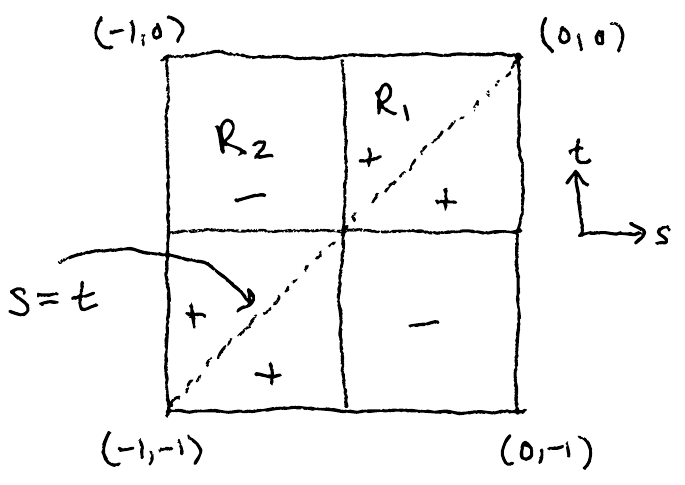
\includegraphics[scale=.6]{region.png}
		\caption{The integral of $|t-s|^{2H}$ over the regions marked with a $+$ are equal. The same goes for those regions marked with a $-$.}
	\end{figure}
\end{solution}

\end{document}